\vspace{10cm}
\subsection{シミュレーション環境}
\subsubsection{計算機性能}
本研究で使用した計算機は,スーパーコンピュータ「京」(以下京, 図\ref{fig:k})と
研究室クラスタ(以下クラスタ, 図\ref{fig:cluster})である. 京はおよそ1京FLOPS(10PFLOPS)の演算性能をもち, 2011年の6月と11月にはTOP500\cite{top500}で世界第1位を,
2017年11月時点では世界第10位を記録している.\\
京の性能諸元\cite{riken-system}を表\ref{table:k}, \ref{table:k-processor}に, クラスタの性能諸元\cite{intel-xeon}を表\ref{table:cluster}に記す.\\

\begin{figure}[htb]
% h:here, t:top, b:bottom, p:page
  \begin{center}
    \includegraphics[width=10.0cm, angle=-90]{./images/k}
    \caption{スーパーコンピュータ京(提供: 理化学研究所)}
    \label{fig:k}
  \end{center}
\end{figure}~\\

\begin{table}[htb]
  \begin{center}
    \caption{京計算ノード構成}
    \begin{tabular}{|p{4cm}|p{10cm}|}
      \hline
      ピーク演算性能 & 10.62PFLOPS \\ \hline
      メモリ総容量 & 1.26PB(ノードあたり16GB)\\ \hline
      計算ノード間ネットワーク & 6次元メッシュ/トーラス(ユーザービューは3次元トーラス)\\ \hline
      帯域 & 3次元の正負各方向にそれぞれ5GB/s×2(双方向)\\ \hline
    \end{tabular}
    \label{table:k}
  \end{center}
\end{table}~\\

\vspace{2cm}
\begin{table}[ht]
  \begin{center}
    \caption{京プロセッサ構成}
    \begin{tabular}{|p{6cm}|p{8cm}|}
      \hline
      CPU性能 & 128GFLOPS(16GFLOPS×8コア)\\ \hline
      コア数 & 8個\\ \hline
      浮動小数点演算器構成(コアあたり)& 積和演算器: 4(2×2個 SIMD), (逆数近似命令: SIMD 動作)除算器: 2個 比較器: 2個\\
      & 浮動小数点レジスタ(64ビット): 256本 グローバルレジスタ(64ビット): 188本\\ \hline
      キャッシュ構成 & 1次命令キャッシュ: 32KB(2way), 1次データキャッシュ: 32KB(2-way), 2次キャッシュ: 6MB(12-way) コア間共有\\ \hline
      メモリ帯域 & 64GB/s(理論ピーク値)\\ \hline
      動作周波数 & 2GHz \\ \hline
      ダイサイズ & 22.7mm × 22.6mm \\ \hline
      トランジスタ数 & 約7億6000万個 \\ \hline
      消費電力 & 58W(プロセス条件TYP)\\ \hline
    \end{tabular}
    \label{table:k-processor}
  \end{center}
\end{table}~\\
\clearpage

\begin{figure}[h]
% h:here, t:top, b:bottom, p:page
  \begin{center}
    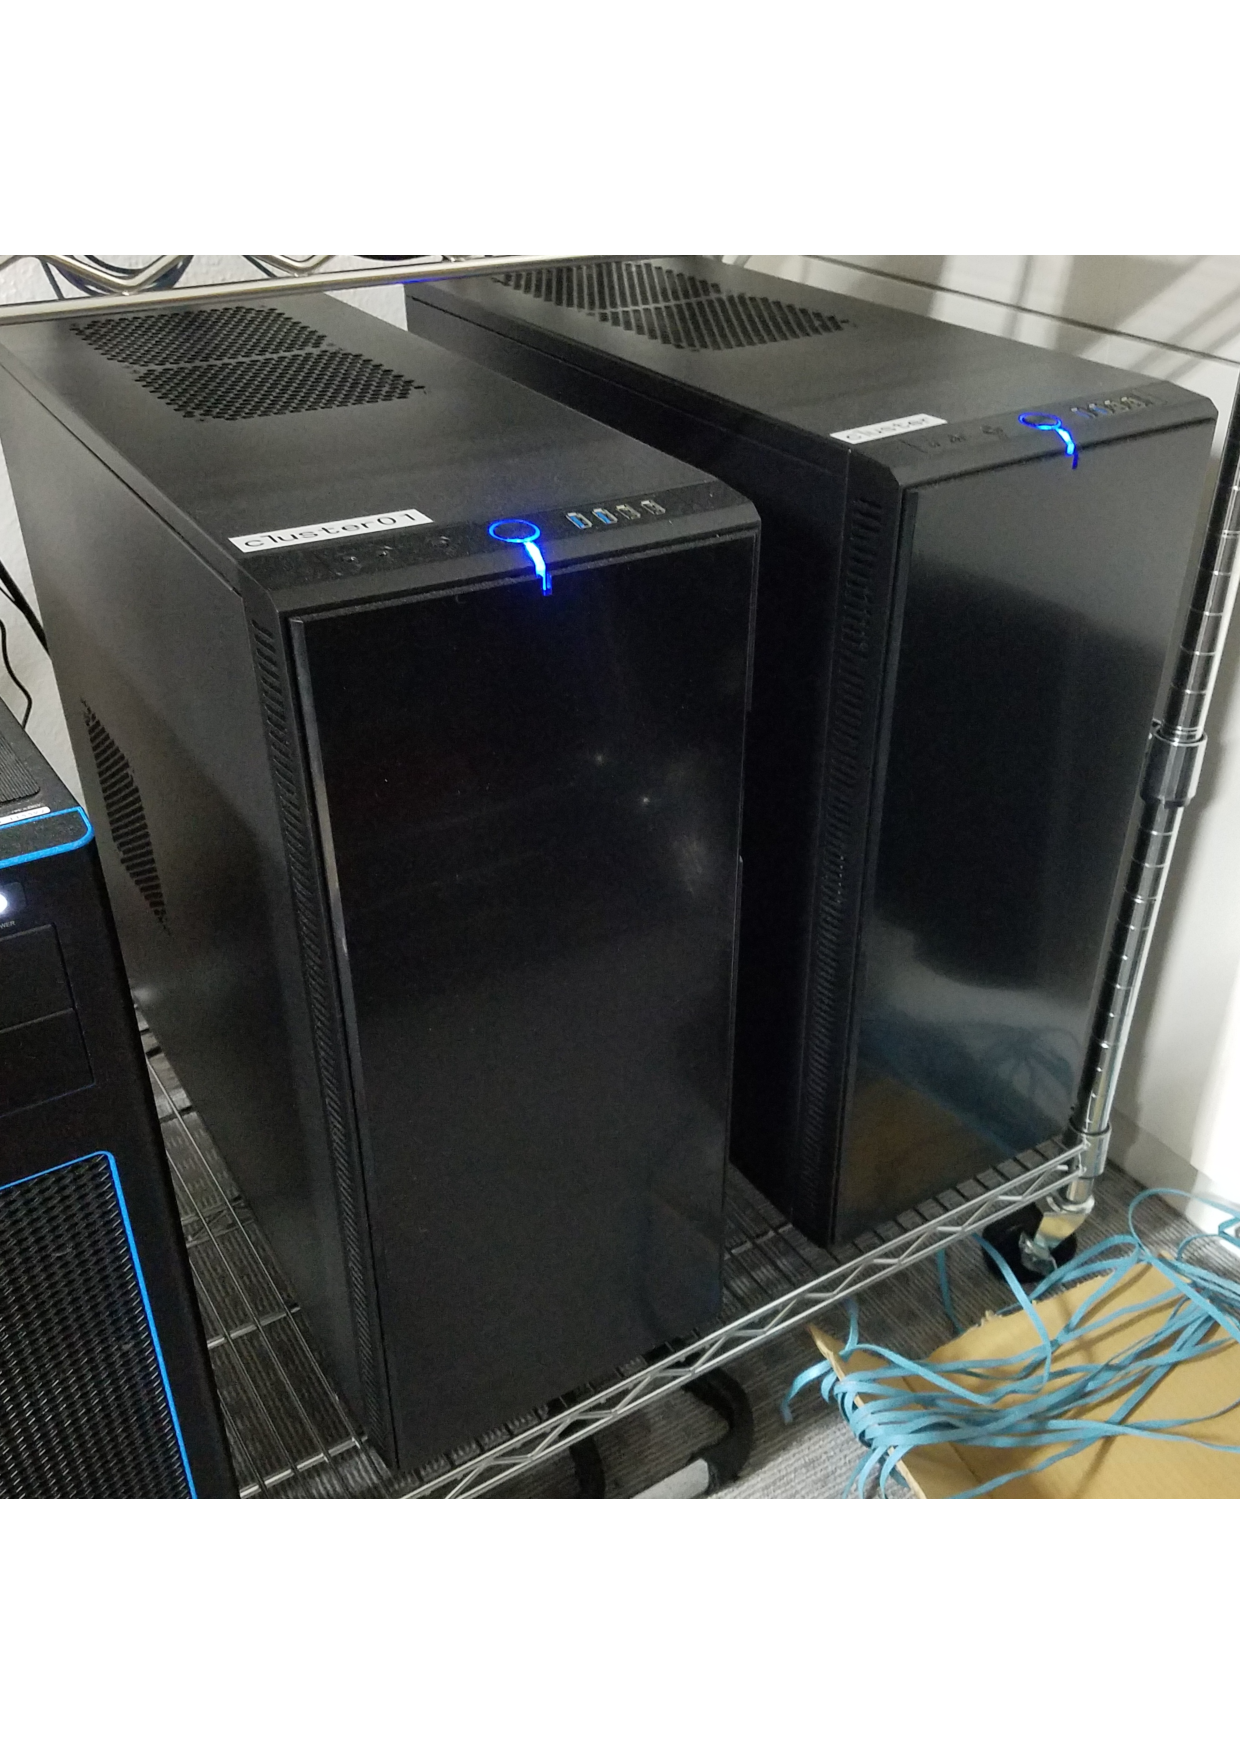
\includegraphics[width=8.0cm]{./images/cluster.pdf}
  \vspace*{-15mm}
  \caption{研究室クラスタ}
  \end{center}
  \label{fig:cluster}
\end{figure}~\\

\begin{table}[hb]
  \caption{クラスタ性能}
  \begin{center}
    \begin{tabular}{|p{4cm}|p{10cm}|}
      \hline
      CPU性能 & 268\.8 GFLOPS(19.2GFLOPS×14コア)\\ \hline
      コア数 & 14コア \\ \hline
      キャッシュ構成 & 1次命令キャッシュ: 448KB(2way), 1次データキャッシュ: 448KB(2-way), 2次キャッシュ: 3.5MB(12-way) コア間共有\\ \hline
      メモリ帯域 & 76.8GB/s(理論ピーク値)\\ \hline
      動作周波数 & 2.4GHz \\ \hline
      消費電力 & 120W\\ \hline
    \end{tabular}
    \label{table:cluster}
  \end{center}
\end{table}~\\

\clearpage
\subsubsection{ジョブ実行環境}
\label{subsec:job-env}
京に代表される大型コンピュータの場合,複数の利用者が共同で利用することが基本となる. そのため各個人が
各々勝手にプログラムを実行すると,計算が集中することで処理限界を大幅に超えてしまったり,逆に全く利用されない時間
などが現れてしまい計算資源を有効に活用できない. 従って, 大型コンピュータではキューイングシステムを利用してプログラムが実行される.\\
キューイングシステムにおける一度のプログラム実行の単位はジョブと呼ばれ,プログラムを実行する際に必要なノード数,メモリ,実行するプログラムのパスや前処理
といった情報を書き込んだジョブスクリプトを作成し,キューイングシステムにジョブスクリプトをサブミットすることでプログラムが実行される.\\
% clusterの説明
\paragraph{クラスタでのジョブの実行}~\\
\begin{table}[htb]
  \caption {クラスタでのジョブ関連コマンド}
  \begin{center}
    \begin{tabular}{|c|p{12cm}|}
      \hline
      コマンド & 説明 \\ \hline
      qsub & qsub \"サブミットするスクリプトのパス\"とすることでジョブをキューシステムに登録し,ジョブIDを出力する.\\ \hline
      qdel & pjdel \"ジョブID\"とすることで現在実行中または待機中のジョブを停止・削除する.\\ \hline
      qstat & 現在実行または待機中のジョブの一覧を表示する\\ \hline
    \end{tabular}
  \end{center}
\end{table}
\clearpage

{\footnotesize
\lstinputlisting[caption=クラスタのジョブスクリプト例, label=cluster-job-script,frame=single]{src/job/cluster-job}
}

{\footnotesize
\begin{lstlisting}[caption=クラスタでのコマンド実行例,label=cluster-job-example,numbers=none]
$ qsub job.sh
20252.cluster.localdomain

$ qstat
>> qstat
Every 1.0s: qstat                                                                                                                                            Wed Jan 10 01:06:06 2018

Job ID                    Name             User            Time Use S Queue
------------------------- ---------------- --------------- -------- - -----
20251.cluster              job.sh        inoue           00:05:38 C cluster
20252.cluster              job.sh        inoue                  0 R cluster
\end{lstlisting}
}

\begin{table}[htb]
  \caption {クラスタでのジョブの状態}
  \begin{center}
    \begin{tabular}{|c|p{12cm}|}
      \hline
      ジョブのステータス & 説明 \\ \hline
      Q & ジョブキューで待機中.\\ \hline
      R & ジョブを実行してる.\\ \hline
      C & ジョブが完了した.\\ \hline
    \end{tabular}
  \end{center}
\end{table}


% kの説明
\paragraph{京でのジョブの実行}~\\
\begin{table}[htb]
  \caption {京でのジョブ関連コマンド}
  \begin{center}
    \begin{tabular}{|c|p{12cm}|}
      \hline
      コマンド & 説明 \\ \hline
      pjsub & pjsub サブミットするスクリプトのパス\\
            & とすることでジョブをキューシステムに登録し,ジョブIDを出力する.\\ \hline
      pjdel & pjdel ジョブID\\
            & とすることで現在実行中または待機中のジョブを停止・削除する.\\ \hline
      pjstat & 現在実行または待機中のジョブの一覧を表示する\\ \hline
    \end{tabular}
  \end{center}
\end{table}

{\footnotesize
\lstinputlisting[caption=京のジョブスクリプト例, label=k-job-script,frame=single]{src/job/k-job}
}

\begin{table}[htb]
  \caption {京でのコマンド実行例}
{\scriptsize
\begin{framed}
\begin{verbatim}
$ pjsub job.sh
[INFO] PJM 0000 pjsub Job 7129316 submitted.

$ pjstat
ACCEPT QUEUED  STGIN  READY RUNNING RUNOUT STGOUT   HOLD  ERROR   TOTAL
    0      1      0      0       0      0      0      0      0       1

JOB_ID   JOB_NAME  MD  ST   USER    GROUP  START_DATE       ELAPSE_TIM  NODE_REQUIRE    RSC_GRP  SHORT_RES
7129316  job.sh    NM  QUE  user    group  [--/-- --:--:--]  0000:00:00      1:-         small    -
\end{verbatim}
\end{framed}
}
\end{table}

\begin{table}[htb]
  \caption {京でのジョブの状態}
  \begin{center}
    \begin{tabular}{|c|p{12cm}|}
      \hline
      ジョブのステータス & 説明 \\ \hline
      QUE & ジョブキューで待機中.\\ \hline
      STI & ジョブの実行に必要なファイルをステージインしている.\\ \hline
      RUN & ジョブを実行中.\\ \hline
      STO & ジョブの実行結果をステージアウトしている.\\ \hline
    \end{tabular}
  \end{center}
\end{table}

